\subsection{Фазовые траектории полномерной модели.}

Не уточняя вид потенциала в гамильтониане \eqref{model_ham2}, система динамических уравнений выглядит следующим образом:

\begin{gather}
\left\{
\begin{aligned}
& \dot{q} = \frac{\partial \mathcal{H}}{\partial p} = \frac{2p}{I_0} + \frac{r_1^2 - r_2^2}{2m r_1^2 r_2^2} J \sin \Phi \sin \Theta \\
& \dot{r_1} = \frac{\partial \mathcal{H}}{\partial p_1} = \frac{p_1}{m} \\
& \dot{r_2} = \frac{\partial \mathcal{H}}{\partial p_2} = \frac{p_2}{m}  \\
& \dot{p} = - \frac{\partial \mathcal{H}}{\partial q} = \frac{J^2 \cos^2 \Phi \sin^2 \Theta \sin q}{2 I_0 (1 - \cos q)^2} - \frac{J^2 \cos^2 \Theta \sin q}{2 I_0 (1 + \cos q)^2} - \frac{r_1^2 - r_2^2}{r_1^2 + r_2^2} \frac{J^2 \cos \Phi \sin \Theta \cos \Theta \cos q}{I_0 \sin^2 q} - \frac{\rmd U}{\rmd q}  \\
& \dot{p_1} = - \frac{\partial \mathcal{H}}{\partial r_1} =
\frac{1}{2} \left[ \frac{J^2 \cos^2 \Phi \sin^2 \Theta}{I_0 (1 - \cos q)} + \frac{J^2 \sin^2 \Phi \sin^2 \Theta}{2 I_0} + \frac{J^2 \cos^2 \Theta}{I_0 (1 + \cos q)} \right] \frac{1}{r_1} \left( 2 - \frac{I_0}{m r_2^2} \right) - \notag \\
& \hspace{1cm} - \frac{J^2 \cos \Phi \sin \Theta \cos \Theta}{I_0 \sin q} \left[ \frac{4 r_1 r_2^2}{(r_1^2 + r_2^2)^2} - \frac{r_1^2 - r_2^2}{r_1^2 + r_2^2} \frac{1}{r_1} \left( 2 - \frac{I_0}{m r_2^2} \right) \right] - \frac{p}{m r_1^3} J \sin \Phi \sin \Theta - \frac{\rmd U}{\rmd r_1} \\
& \dot{p_2} = - \frac{\partial \mathcal{H}}{\partial r_2} = 
\frac{1}{2} \left[ \frac{J^2 \cos^2 \Phi \sin^2 \Theta}{I_0 (1 - \cos q)} + \frac{J^2 \sin^2 \Phi \sin^2 \Theta}{2 I_0} + \frac{J^2 \cos^2 \Theta}{I_0 (1 + \cos q)} \right] \frac{1}{r_2} \left( 2 - \frac{I_0}{m r_1^2} \right) + \notag \\
& \hspace{1cm} + \frac{J^2 \cos \Phi \sin \Theta \cos \theta}{I_0 \sin q} \left[ \frac{4 r_1^2 r_2}{(r_1^2 + r_2^2)^2} + \frac{r_1^2 - r_2^2}{r_1^2 + r_2^2} \frac{1}{r_2} \left( 2 - \frac{I_0}{m r_1^2} \right) \right] + \frac{p}{m r_2^3} J \sin \Phi \sin \Theta - \frac{\rmd U}{\rmd r_2} \\
& \dot{\Phi} = \left[ \left( \frac{J \cos \Phi \sin \Theta}{I_0 (1 - \cos q)} +  \frac{r_1^2 - r_2^2}{r_1^2 + r_2^2} \frac{J \cos \Theta}{I_0 \sin q} \right) \cos \Phi + \left( \frac{J \sin \Phi \sin \Theta}{2 I_0} + \frac{r_1^2 - r_2^2}{2 m r_1^2 r_2^2} p \right) \sin \Phi \right] \ctg \Theta - \notag \\
& \hspace{3cm} - \left( \frac{J \cos \Theta}{I_0 ( 1 + \cos q)} + \frac{r_1^2 - r_2^2}{r_1^2 + r_2^2} \frac{J \cos \Phi \sin \Theta}{I_0 \sin q} \right) \\
& \dot{\Theta} = \left( \frac{J \cos \Phi \sin \Theta}{I_0 ( 1 - \cos q)} + \frac{r_1^2 - r_2^2}{r_1^2 + r_2^2} \frac{J \cos \Theta}{I_0 \sin q} \right) \sin \Phi - \left( \frac{J \sin \Phi \sin \Theta}{2 I_0} + \frac{r_1^2 - r_2^2}{2m r_1^2 r_2^2} p \right) \cos \Phi 
\end{aligned}
\right. \notag
\end{gather}
 
Решение представленной системы дифференциальных уравнений с потенциалами, описанными выше, производилось при помощи математической платформы \textit{Maple 2015}. 

Построим схему определения начальных условий, аналогичную описанной для более простой модельной системы. Первым шагом необходимо задаться значениями энергетических уровней соответствующих потенциалов. Обозначим $n$ -- уровень возбуждения деформационного колебания, $E_n$ -- энергия соответствующего уровня; $n_1$, $n_2$ -- уровни возбуждения валентных колебаний, $E_{n_1}$, $E_{n_2}$ -- энергии соответствующих уровней. Найдем эффективный потенциал и используем тот факт, что гамильтониан является интегралом движения:
\vverh
\begin{gather}
V_{eff.} = \frac{1}{2} \vec{J}^{\, \top} \bbI^{-1} \vec{J} + U(q, r_1, r_2) \notag \\
V_{eff.} = \frac{J_x^2}{2 I_0 (1 - \cos q)} + \frac{J_y^2}{m (r_1^2 + r_2^2)} + \frac{J_z^2}{I_0 (1 + \cos q)} + \frac{r_1^2 - r_2^2}{r_1^2 + r_2^2} \frac{J_x J_z}{2I_0 \sin q} + U(r_1, r_2, q) \notag \\
E_n + E_{n_1} + E_{n_2} = V_{eff.}(r_{1,0}, r_{2,0}, q_0, \Theta_0, \Phi_0) + \frac{r_{1,0}^2 - r_{2,0}^2}{r_{1,0}^2 + r_{2,0}^2} \frac{J_{y,0}^2}{4 m r_{1,0}^2 r_{2,0}^2} + \frac{r_{1,0}^2 - r_{2,0}^2}{2m r_{1,0}^2 r_{2,0}^2} J_{y,0} p_0 + \frac{p_{1,0}^2}{2m} + \frac{p_{2,0}^2}{2m} + \frac{p_0^2}{I_0} \notag \\
\left\{
\begin{aligned}
J_{x,0} &= J \cos \Phi_0 \sin \Theta_0 \\
J_{y,0} &= J \sin \Phi_0 \sin \Theta_0 \\
J_{z,0} &= J \cos \Theta_0
\end{aligned}
\right. \notag
\end{gather}

Заметим, что если мы возьмем $\Phi_0 = 0$, то $J_{y, 0} = 0$, и полученное выражение значительно упростится. Также положим $p_{1,0} = p_{2,0} = 0$, что дополнительно упростит выражение.
Приходим к выражению, аналогичному тому, что было выписано для предыдущей модельной системы:
\vverh
\begin{gather}
E_n + E_{n_1} + E_{n_2} = V_{eff.}(r_{1,0}, r_{2,0}, q_0, \Theta_0, \Phi_0) + \frac{p_0^2}{I_0}
\label{three_energy}
\end{gather}

Используя полуклассический подход, определим начальные значения $r_{1, 0}$, $r_{2, 0}$, при которых энергии валентных колебаний равны $E_{n_1}$ и $E_{n_2}$, соответственно. В случае гармонического потенциала начальное значение длины связи может быть получено в аналитической форме:  $r_1 = r_0 \pm \sqrt{\ddfrac{E_{n_1}}{k}}$, но в случае потенциала Морзе -- только численными методами. 
В качестве начального значения угла $q_0$ возьмем $q_e$, которое определяется модулем вектора углового момента и его направлением (выражение \eqref{eq_angle}). Таким образом, нам осталось определить начальное значение импульса $p$, которое мы находим исходя из соотношения \eqref{three_energy}, предварительно рассчитав значение эффективного потенциала при заданных условиях (не забывая про то, что $I_0 = I_0 (r_{1,0}, r_{2,0})$).
\vverh
\begin{gather}
p = \sqrt{I_0 (E_n + E_{n_1} + E_{n_2} - V_{eff.} (q_0, r_{1,0}, r_{2,0}, \Theta_0, \Phi_0))} \notag
\end{gather}

Построим траектории вектора углового момента для обеих модельных систем. Как и при построении траекторий для прошлой модели, будем изображать их на сферах одинакового радиуса. Для всех траекторий было взято начальное значение сферического угла $\Theta = 0.3 \text{рад.}$. Изучим классические траектории для модельной системы с валентным потенциалом гармонического типа в основном колебательном состоянии ($n = 0$, $n_1 = 0$, $n_2 = 0$).

\vverh
\begin{figure}[H]
  \begin{center}
    \begin{tikzpicture}[framed, ->, >=stealth', auto, thick]
    
      \tikzstyle{type1} = [rectangle, rounded corners, minimum width = 3cm, minimum height = 1cm, text centered, text width = 3cm ,draw = black, fill = red!30]

\tikzstyle{type2} = [rectangle, rounded corners, minimum width = 3cm, minimum height = 1cm, text centered, text width = 3cm, draw = black, fill = green!30]

\tikzstyle{type3} = [rectangle, rounded corners, minimum width = 3cm, minimum height = 1.5cm, text centered, text width = 5 cm, draw = black, fill = yellow!30]

\tikzstyle{arrow} = [thick, ->, >=stealth]

\node (n) [type2] {$n$};
\node (n1) [type2, right = 0.5 cm of n] {$n_1$};
\node (n2) [type2, right = 0.5 cm of n1] {$n_2$};
\node (n_container) [type3, fit = (n) (n1) (n2)] {};
\node (n) [type2] {$n$};
\node (n1) [type2, right = 0.5 cm of n] {$n_1$};
\node (n2) [type2, right = 0.5 cm of n1] {$n_2$};

\node (r2) [type1, below right = 1 cm and 2 cm of n_container] {$r_{2,0}$};
\node (r1) [type1, below = 0.5 cm of r2] {$r_{1,0}$};
\node (r_container) [type3, fit = (r1) (r2)] {};	
\node (r2) [type1, below right = 1 cm and 2 cm of n_container] {$r_{2,0}$};
\node (r1) [type1, below = 0.5 cm of r2] {$r_{1,0}$};

\node (theta) [type2, below = 5.5 cm of n_container] {$\Theta_0$};
\node (phi) [type2, right = 1 cm of theta] {$\Phi_0 = 0$};
\node (angle_container) [type3, fit = (theta) (phi)] {}; 
\node (theta) [type2, below = 5.5 cm of n_container] {$\Theta_0$};
\node (phi) [type2, right = 1 cm of theta] {$\Phi_0 = 0$};

\node (energy) [type2, below left = 5.5 cm and 0.5 cm of n_container] {$E = E_n + E_{n_1} + E_{n_2}$};

\path (n1) edge[bend right] node [left] {} (r1);
\path (n2) edge[bend right] node [left] {} (r2); 
      
	  \begin{scope}[on background layer]
  		\node (outer) [draw,fill = gray!30, fit = (n_container) (r_container) (angle_container) (energy) (q) (J)] {};
  	  \end{scope}
    \end{tikzpicture}
    \caption{Схема определения начальных параметров системы.}
  \end{center}
\end{figure}

Заметим, что при малых значениях момента фазовая траектория имеет достаточно сложный профиль, значительно отличающийся от эллиптического прецессионого профиля, который мы наблюдали для модели с деформационным потенциалом. С ростом модуля вектора углового момента профиль фазовой траектории усложняется, выделяются циклические структуры в окрестности тех положений, где ожидается возникновение новых устойчивых осей вращения. Однако образования характерных участков фазовых траекторий, указывающих на наличие особой точки типа центр, не происходит. Лишь при достижении значительно более высокого значения момента ($J = 26$) происходит локализация траектории вокруг новой устойчивой оси вращения.

\begin{figure}[H]
  \centering
	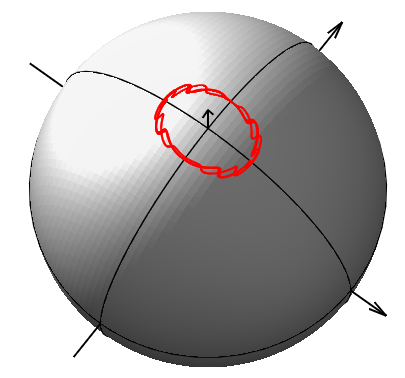
\includegraphics[width=0.15\textwidth]{../pictures/HarmGroundState00/plot_J=10.png}
	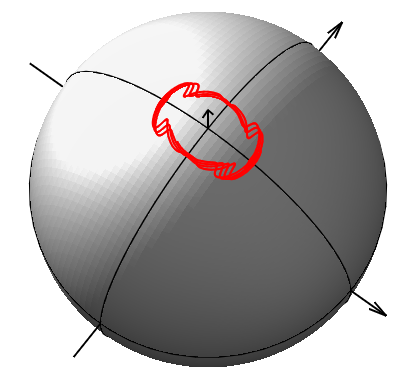
\includegraphics[width=0.15\textwidth]{../pictures/HarmGroundState00/plot_J=15.png}
	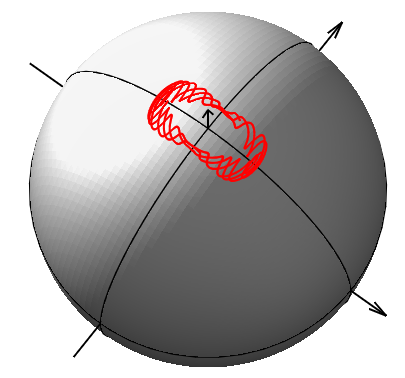
\includegraphics[width=0.15\textwidth]{../pictures/HarmGroundState00/plot_J=20.png}
	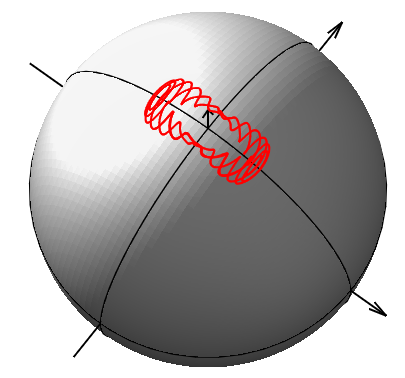
\includegraphics[width=0.15\textwidth]{../pictures/HarmGroundState00/plot_J=22.png}
	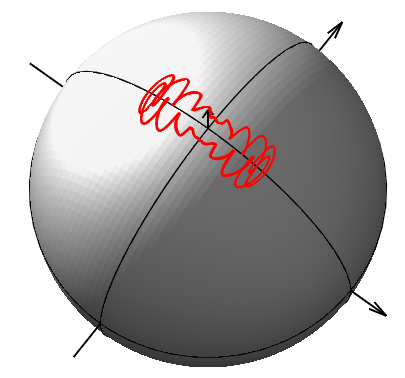
\includegraphics[width=0.15\textwidth]{../pictures/HarmGroundState00/plot_J=24.png}
	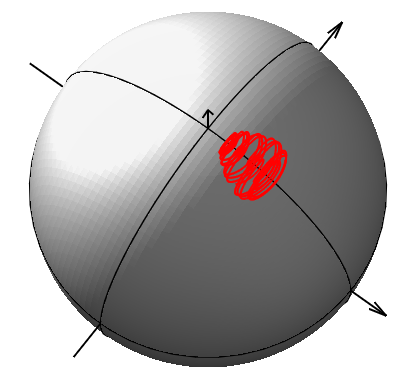
\includegraphics[width=0.15\textwidth]{../pictures/HarmGroundState00/plot_J=26.png}
	\caption{Динамика вектора углового момента полной модельной системы с валентным потенциалом гармонического типа в основном колебательном состоянии ${n = 0, n_1 = 0, n_2 = 0}$. Модуль вектора углового момента: $J = 10, \, 15, \, 20, \, 22, \, 24, \, 26$.} 
	\label{fig:harm000}
\end{figure}

Посмотрим какое влияние оказывает значение энергетического уровня на проявление бифуркациии и профиль фазовой траектории. Изменим энергетический уровень одного валентного колебания с основного на первый. Уже при малых значениях модуля вектора углового момента ощущается наблюдается заметная асимметричность фазовой траектории, усиливающая с увеличением углового момента системы. Отметим, что точный момент бифуркации по такого сорта фазовым траекториям установить сложно. Однако полная локализация фазовой траекторий вокруг новой устойчивой оси вращения происходит при значениях углового момента системы уже на несколько единиц меньше тех значений, при которых наблюдалась подобная локализация для системы в основном колебательном состоянии. Траектории, представленные на рисунке \eqref{fig:harm050} подтверждают высказанное замечание. На рисунке  \eqref{fig:harm050} изображены траектории, соотвествующие модельной системе с колебательным возбуждением $\left\{ n = 0, n_1 = 5, n_2 = 0 \right\}$. Помимо ярко выраженной асимметричности профиля фазовой траектории и заметного его усложнения с ростом углового момента, полная локализация траектории вокруг новой оси устойчивого вращения наблюдается уже при значении $J = 20$.

\begin{figure}[H]
  \centering
	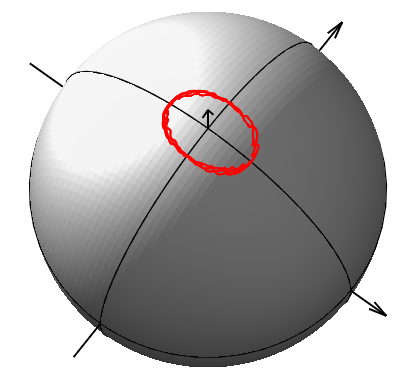
\includegraphics[width=0.15\textwidth]{../pictures/HarmGroundState10/plot_J=10.png}
	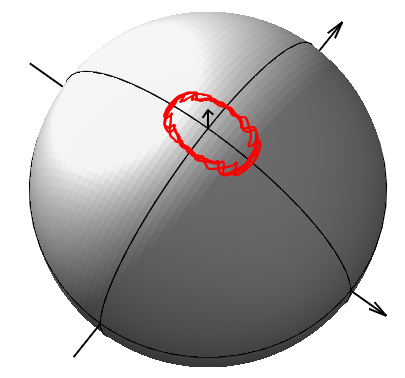
\includegraphics[width=0.15\textwidth]{../pictures/HarmGroundState10/plot_J=15.png}
	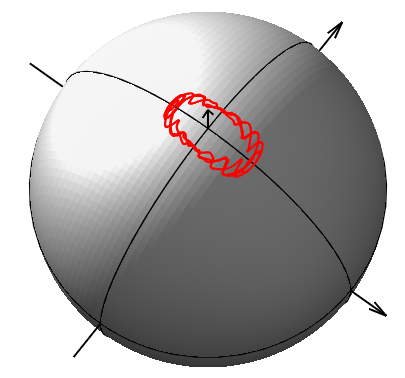
\includegraphics[width=0.15\textwidth]{../pictures/HarmGroundState10/plot_J=18.png}
	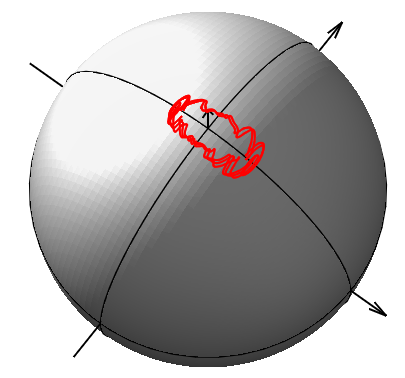
\includegraphics[width=0.15\textwidth]{../pictures/HarmGroundState10/plot_J=20.png}
	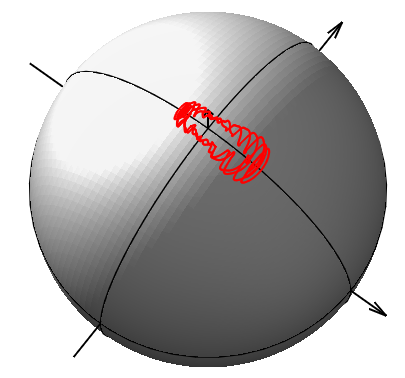
\includegraphics[width=0.15\textwidth]{../pictures/HarmGroundState10/plot_J=22.png}
	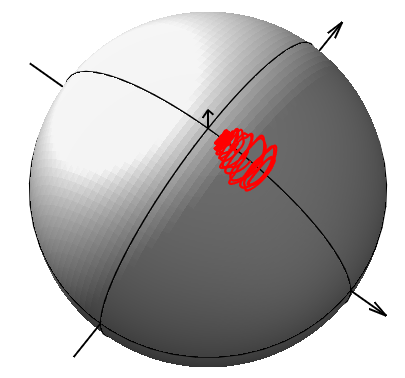
\includegraphics[width=0.15\textwidth]{../pictures/HarmGroundState10/plot_J=24.png}
	\caption{Динамика вектора углового момента полной модельной системы с валентным потенциалом гармонического типа в колебательном состоянии $\left\{ n = 0, n_1 = 1, n_2 = 0 \right\}$. Модуль вектора углового момента: $J = 10, \, 15, \, 18, \, 20, \, 22, \, 24$.}
\label{fig:harm010}
\end{figure}


\begin{figure}[H]
  \centering
	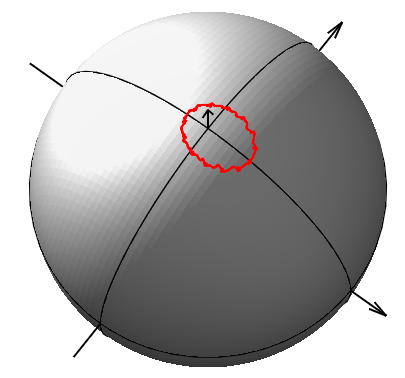
\includegraphics[width=0.15\textwidth]{../pictures/HarmGroundState50/plot_J=5.png}
	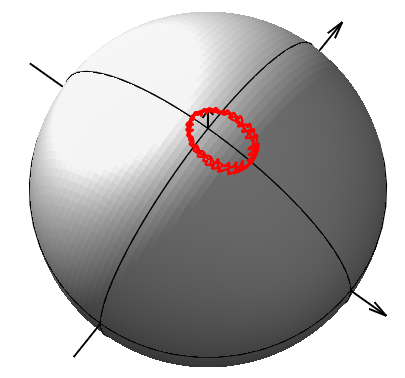
\includegraphics[width=0.15\textwidth]{../pictures/HarmGroundState50/plot_J=10.png}
	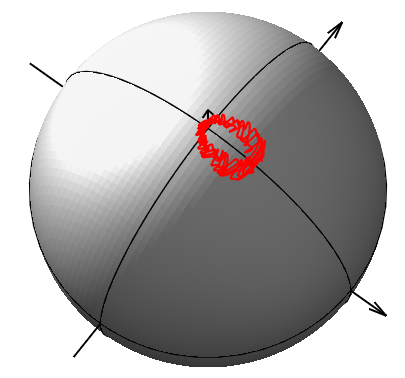
\includegraphics[width=0.15\textwidth]{../pictures/HarmGroundState50/plot_J=15.png}
	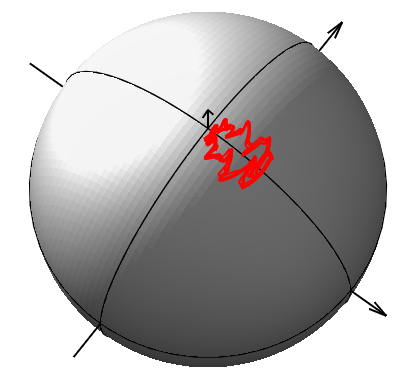
\includegraphics[width=0.15\textwidth]{../pictures/HarmGroundState50/plot_J=18.png}
	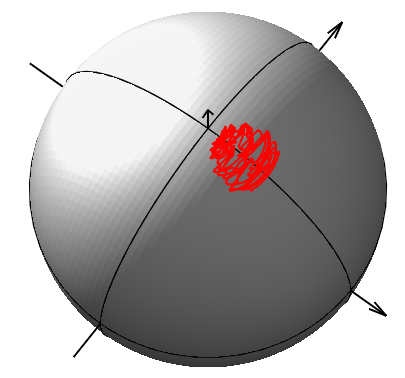
\includegraphics[width=0.15\textwidth]{../pictures/HarmGroundState50/plot_J=20.png}
	\caption{Динамика вектора углового момента полной модельной системы с валентным потенциалом гармонического типа в колебательном состоянии $\left\{ n = 0, n_1 = 5, n_2 = 0 \right\}$. Модуль вектора углового момента: $J = 5, \, 10, \, 15, \, 18, \, 20$.}	
\label{fig:harm050}
\end{figure}

Проанализируем влияние, оказываемое уровнем деформационного возбуждения на положение бифуркации для модельной системы с потенциалом гармонического типа. На рисунке \eqref{ham200} представлены траектории, соответствующие системы с колебательным возбуждением $\left\{ n = 2, n_1 = 0, n_2 = 0 \right\}$. С ростом углового момента системы, как и в предыдущих случаях, происходит усложнение профиля траектории, сопровождающееся уменьшением фазовой локализации. Однако "перескакивания" траектории, наблюдаемого в основном колебательном состоянии не наблюдается вплоть до $J = 30$ (и даже после "перескакивания" траектория не обладает пространственной локализацией). 

\begin{figure}[H]
  \centering
	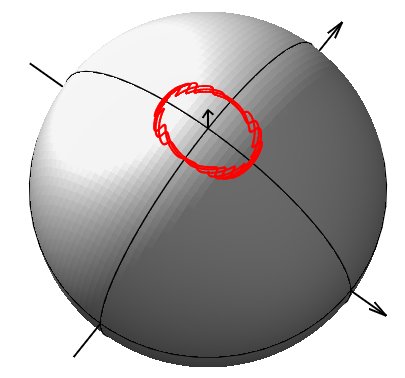
\includegraphics[width=0.15\textwidth]{../pictures/HarmSecondState00/plot_J=10.png}
	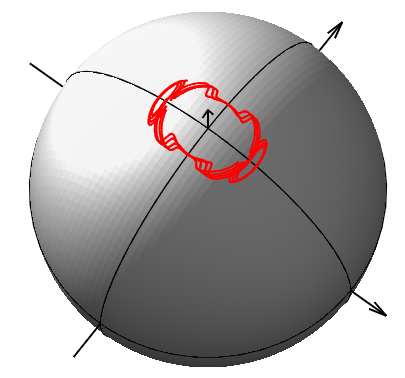
\includegraphics[width=0.15\textwidth]{../pictures/HarmSecondState00/plot_J=15.png}
	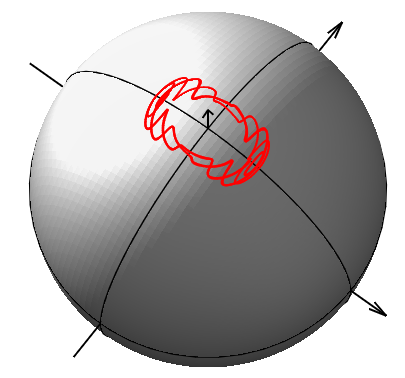
\includegraphics[width=0.15\textwidth]{../pictures/HarmSecondState00/plot_J=18.png}
	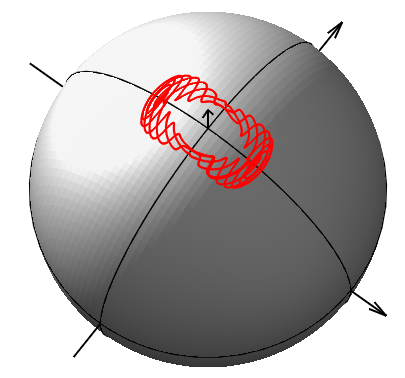
\includegraphics[width=0.15\textwidth]{../pictures/HarmSecondState00/plot_J=20.png}
	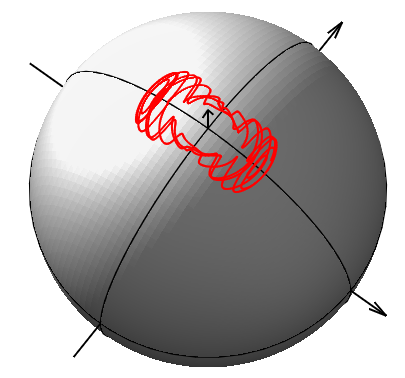
\includegraphics[width=0.15\textwidth]{../pictures/HarmSecondState00/plot_J=22.png}
	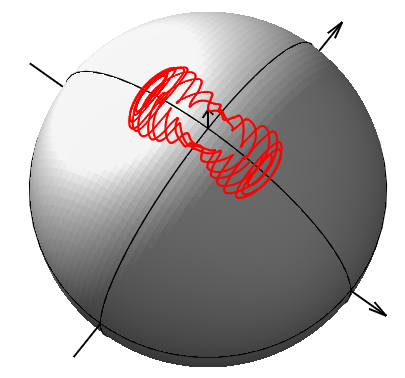
\includegraphics[width=0.15\textwidth]{../pictures/HarmSecondState00/plot_J=24.png}
	\caption{Динамика вектора углового момента полной модельной системы с валентным потенциалом гармонического типа в колебательном состоянии $\left\{ n = 2, n_1 = 0, n_2 = 0 \right\}$. Модуль вектора углового момента: $J = 10, \, 15, \, 18, \, 20, \, 22, \, 24$.}
\label{ham200}
\end{figure}

Увеличение энергетического уровня колебания деформационного типа не приводит к однозначному изменению положения бифуркации; при этом фазовая локализация траекторий значительно уменьшается. \\
Проследим описанные закономерности на второй модельной системе, в которой валентные колебания описываются потенциалом Морзе. Профиль полученных траекторий уже в основном колебательном состоянии оказывается значительно сложнее тех, что были получены для двух предыдущих моделей. Заметим, что выбор реалистического валентного потенциала сместил положение бифуркации в еще большие значения углового момента. В основном колебательном состоянии наблюдается бифуркация при $J \approx 29-30$.

\begin{figure}[H]
  \centering
	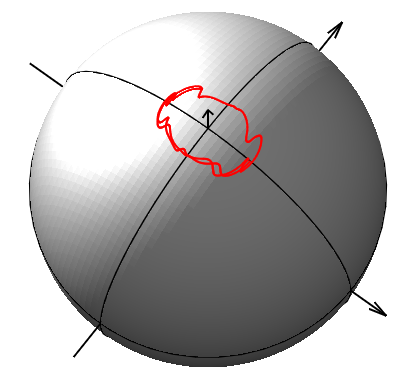
\includegraphics[width=0.15\textwidth]{../pictures/MorseGroundState00/plot_J=15.png}
	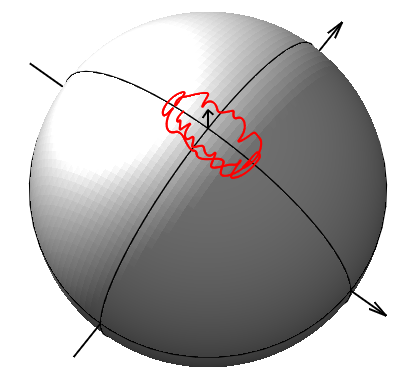
\includegraphics[width=0.15\textwidth]{../pictures/MorseGroundState00/plot_J=20.png}
	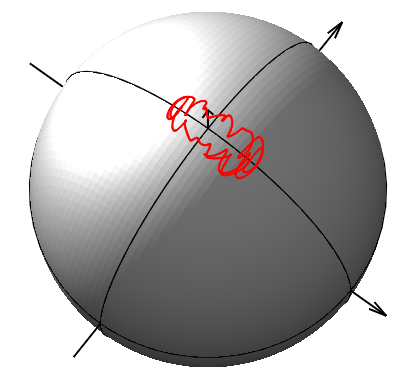
\includegraphics[width=0.15\textwidth]{../pictures/MorseGroundState00/plot_J=25.png}
	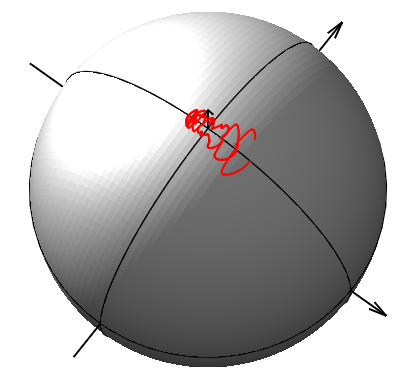
\includegraphics[width=0.15\textwidth]{../pictures/MorseGroundState00/plot_J=28.png}
	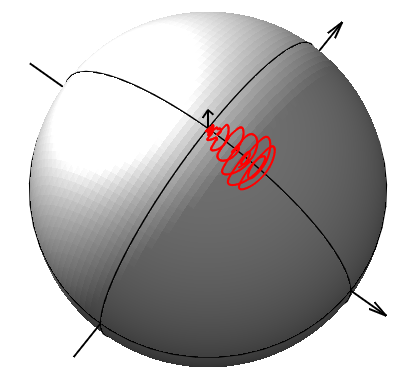
\includegraphics[width=0.15\textwidth]{../pictures/MorseGroundState00/plot_J=29.png}
	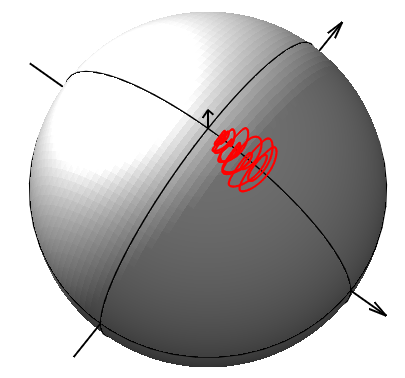
\includegraphics[width=0.15\textwidth]{../pictures/MorseGroundState00/plot_J=30.png}
	\caption{Динамика вектора углового момента полной модельной системы с валентным потенциалом Морзе в колебательном состоянии $\left\{ n = 0, n_1 = 0, n_2 = 0 \right\}$. Модуль вектора углового момента: $J = 15, \, 20, \, 25, \, 28, \, 29, \, 30$.} 
\label{fig:morse000}
\end{figure}

Проследим за тем, как будет изменяться положение бифуркации с ростом энергетического уровня валентного колебания. На рисунке \eqref{fig:morse030} приведены фазовые траектории системы в колебательном состоянии $\left\{ n = 0, n_1 = 3, n_2 = 0 \right\}$.  Уже при значении момента $J = 10$ происходит локализации траектории вокруг новой оси, хотя ее направление при данном угловом моменте очень незначительно отклонено от старой оси. То есть, фазовые траектории модели с потенциалом Морзе проявляют значительно большую чувствительность к энергетическому уровню колебаний валентного типа, чем модель с потенциалом гармонического типа.

\begin{figure}[H]
  \centering
	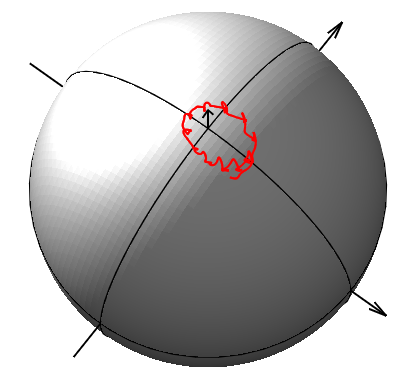
\includegraphics[width=0.15\textwidth]{../pictures/MorseGroundState03/plot_J=6.png}
	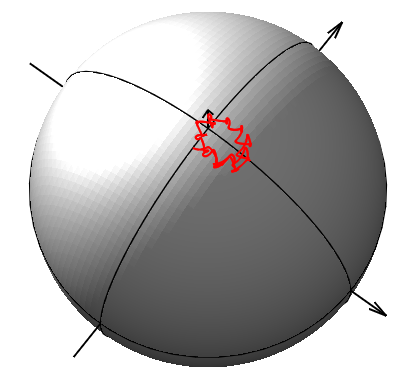
\includegraphics[width=0.15\textwidth]{../pictures/MorseGroundState03/plot_J=8.png}
	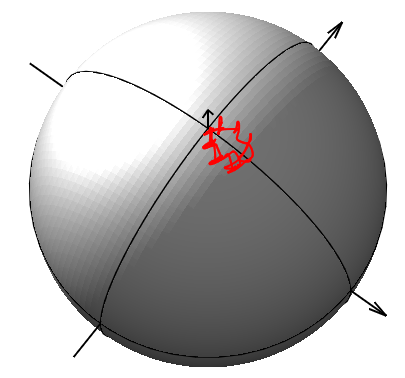
\includegraphics[width=0.15\textwidth]{../pictures/MorseGroundState03/plot_J=10.png}
	\caption{Динамика вектора углового момента полной модельной системы с валентным потенциалом Морзе в колебательном состоянии $\left\{ n = 0, n_1 = 3, n_2 = 0 \right\}$. 
Модуль вектора углового момента: $J = 6, \, 8, \, 10$.}
\label{fig:morse030}
\end{figure}

На рисунке \eqref{fig:morse200} представлены фазовые траектории системы в состоянии $\left\{ n = 2, n_1 = 0, n_2 = 0 \right\}$. Несмотря на то что при средних значениях углового момента системы в фазовых траекториях наблюдается частичная локализация вокруг новых осей вращения, при высоких значениях момента ($J = 25$ и больших) локализация практически теряется. 
 
\begin{figure}[H]
  \centering
	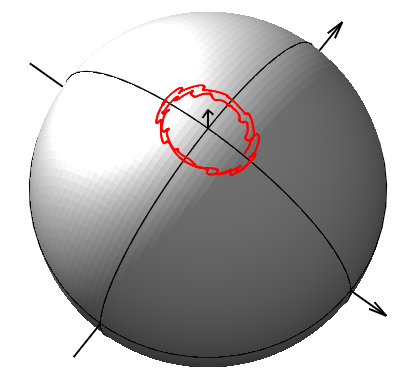
\includegraphics[width=0.15\textwidth]{../pictures/MorseSecondState00/plot_J=5.png}
	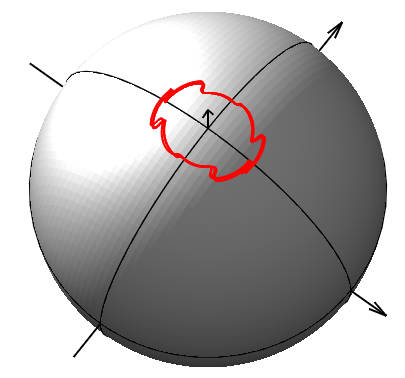
\includegraphics[width=0.15\textwidth]{../pictures/MorseSecondState00/plot_J=10.png}
	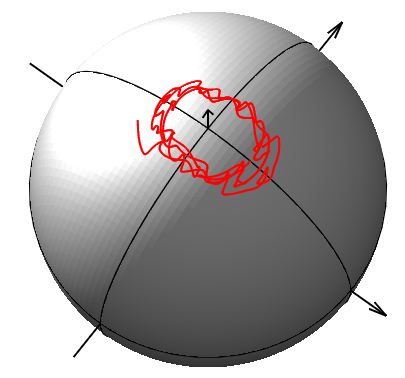
\includegraphics[width=0.15\textwidth]{../pictures/MorseSecondState00/plot_J=15.png}
	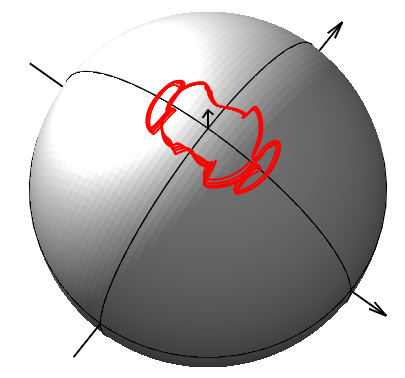
\includegraphics[width=0.15\textwidth]{../pictures/MorseSecondState00/plot_J=20.png}
	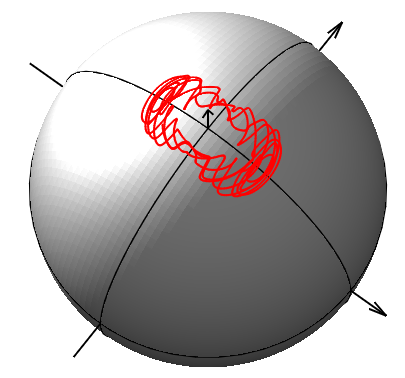
\includegraphics[width=0.15\textwidth]{../pictures/MorseSecondState00/plot_J=25.png}
	\caption{Динамика вектора углового момента полной модельной системы с валентным потенциалом Морзе в колебательном состоянии $\left\{ n = 2, n_1 = 0, n_2 = 0 \right\}$. 
Модуль вектора углового момента: $J = 5, \, 10, \, 15, \, 20, \, 25$.}
\label{fig:morse200}
\end{figure}